% {{{ CYCLE HAMILTONIEN

Au cours de cette section nous nous intéresserons uniquement à l'étape $3$ du schéma de programmation
dynamique classique sur les décompositions arborescentes, ainsi nous supposerons connus $\Taugstar$
et $k$ la largeur de $\mathcal{T}_G^*$.

Comme souligné précédemment, les solutions sont stockées dans des tables. L'encodage des sous
problèmes et donc des solutions partielles sera étudiée à la section~\ref{hcpd_table}. Puis, les
rouages de l'algorithme seront dévoilés en section~\ref{hcpd_action} lorsque nous étudierons comment
une solution partielle est calculée à partir des fils du sac examiné. Dans les deux dernières
parties, nous nous attacherons à démontrer la validité de l'algorithme et calculerons sa
complexité.

%% {{{ REPRESENTATION DES DONNEES ET TAILLE DE LA TABLE
\section{Représentation des solutions partielles}
\label{hcpd_table}

Considérons un graphe $G=(V, E)$ et une décomposition arborescente enracinée et simple de $G$,
$\Taugstar$ de largeur $k$.
\begin{nlemma}
    Si $t_i$ est un sac interne de $T$ et si $H$ est un chemin Hamiltonien dans $G$, alors
    $H[V_{t_i}]$ est une collection de chemins disjoints dont les extrêmités appartiennent à
    $X_{t_i}$.
\end{nlemma}

\begin{proof}
    Considérons un sac interne $t \in T$ tel que $H[V_t]$ possède au moins un chemin $c$ dont au moins
    une extrêmité n'appartient pas à $X_t$. Appelons $v$ l'extrêmité de $c$, par
    hypothèse, $v \not \in X_t$.

    Il y a donc deux possibilités pour $v$ :
    \begin{enumerate}
        \item $v \in G_t$, alors le degré de $v$ dans $H[V_t] = 1$ et donc le degré de $v$ dans $H$
            est aussi égal à $1$, donc $v$ n'appartient pas à un cycle Hamiltonien ce qui soulève une
            contradiction
        \item donc $v \in V\backslash V_t$, par hypothèse $v$ est l'extrêmité d'un chemin appartenant à
            $H[V_t]$, ce qui implique qu'il existe $u \in V_t$ tel que $(uv)$ est un sous-chemin de
            $c$, ayant une extrêmité dans $V_t$ et l'autre dans $V\backslash V_t$ et ne possèdant aucun
            sommet appartenant à $X_t$. Or la proposition~\ref{nsep} nous dit que $X_t$ est un
            séparateur de $G$, ce qui nous amène encore à une contradiction.
    \end{enumerate}
    L'hypothèse de départ est donc fausse.
\end{proof}

On peut se faire une idée du lemme précédent à l'aide des figures~\ref{hcpd_h1}
et~\ref{hcpd_h2}.

En observant la figure~\ref{hcpd_h2}, on se rend compte, qu'il est possible de classifier les
sommets de $X_t$ en trois catégories selon leur degré dans $H[V_t]$ :
\begin{enumerate}
    \item les sommets de degré $2$ dans $H[V_T]$ sont les sommets de $X_t$ pour lesquels, leurs
        deux voisins dans $H$ ont été découverts. Ils seront appelés les sommets internes et seront
        notés $X_t^2$. Il est important de remarquer que pout tout $v \in X_t^2$, les voisins de $v$
        dans $H$ appartiennent à $V[t]$. Ils sont représentés en vert sur la figure~\ref{hcpd_h2}.
    \item les sommets de degré $0$ dans $H[V_T]$ sont les sommets de $X_t$ pour lesquels aucun
        voisin n'a encore été découvert. Nous les appellerons les sommets isolés et les noterons
        $X_t^0$, leurs voisins appartiennent tous deux à $V\backslash V_t$. Ils sont représentés en noir sur
        la figure~\ref{hcpd_h2}.
    \item les sommets de degré $1$ dans $H[V_T]$ sont tous les autres sommets pour lesquels un seul
        de leurs voisin a été découvert, ils représentent l'ensemble des extrêmités de tous les
        chemins de la collection $H[V_t]$. Nous les appellerons les sommets extrémités et les
        noterons $X_t^1$
\end{enumerate}

\begin{nlemma}
    Les ensembles $X_t^0$, $X_t^1$ et $X_t^2$ définissent une partition des sommets de $G$ contenus
    dans $X_t$.
\end{nlemma}

\begin{proof}
    Tous les sommets de $X_t$ sont de degré inférieur ou égal à $2$ dans $H[V_t]$, ce parce que $H$
    est un chemin Hamiltonien ce qui implique que dans $H$ tous les sommets de $X_t$ sont de degré
    $2$, donc $(X_t^0, X_t^1, X_t^2)$ couvre l'ensemble des sommets de $X_t$.

    De plus, un sommet ne peut avoir deux degrés différents, ce qui implique que $X_t^0 \cap X_t^1 =
    X_t^1 \cap X_t^2 = X_t^0 \cap X_t^2 = \emptyset$.

    Il s'agit donc bien d'une partition.
\end{proof}

\begin{ncorol}
    \label{hcpd_ntrip}
    Le nombre de triplets $(X_t^0, X_t^1, X_t^2)$ pour un $X_t$ donné est borné supérieurement par
    $3^{|X_t|}$.
\end{ncorol}

Seulement ces trois seuls ensembles ne suffisent pas à décrire de manière unique une solution
réalisable pour le sac $X_t$. Les deux schémas de la figure~\ref{hcpd_h3} présentent le même triplet
d'ensembles $(X_t^0, X_t^1, X_t^2)$, les collections de chemins ne sont pas identiques.

C'est pourquoi, il faut ajouter un couplage $M$ sur $X_t^1$ à ce triplet liant les deux extrêmités d'un même chemin
dans $X_t$. Considérons par exemple un sac $X_t = \{1, 2, \dots, 7\}$, la représentation de sa
soltution partielle définie par : \[
    (X_t^0 = \{1\}, X_t^1 = \{2, 3, 5, 7\}, X_t^2 = \{4, 6\}, M = \{(2,3), (5,7)\})
\] est donnée à la figure~\ref{hcpd_h4}.

Par la suite, le quadruplet $\pdsol{t}$ désignera, par abus de langage, tantôt le sous problème
associé à $t$ consistant à savoir s'il existe une collection de chemins disjoints de $G_t$ couvrant
l'ensemble des sommets de $V_t$, tantot la solution partielle à ce sous problème.

Et donc pour chaque sac $t$ de la décomposition arborscente, il faut savoir si $(X_t^0, X_t^1,
X_t^2, M)$ est une solution partielle ou non.

\begin{nrmq}
    \label{hcpd_ncoup}
    Le nombre de couplages possibles pour un sac $t$ donné est borné supérieurement par $|X_t|!$
\end{nrmq}

\begin{nlemma}
    Pour un sac $t$ de la décompostion arborescente, il y a $3^{k+1} k!$ sous-problèmes.
\end{nlemma}

\begin{proof}
    Étant donné un graphe $G=(V,E)$ et une décomposition arborescente enracinée simple de $G$
    $\Taugstar$ de largeur $k$. Par définition de la largeur arborescente, $\forall t \in T,\ |X_t|
    \leq k + 1$, donc d'après le corollaire~\ref{hcpd_ntrip} et la remarque~\ref{hcpd_ncoup}, on a : \[
        \forall t \in T,\quad \#((X_t^0, X_t^1, X_t^2, M)) \leq 3^{k+1} k!
    \]
\end{proof}

% {{{ FIGURES
\begin{figure}
    \begin{center}
        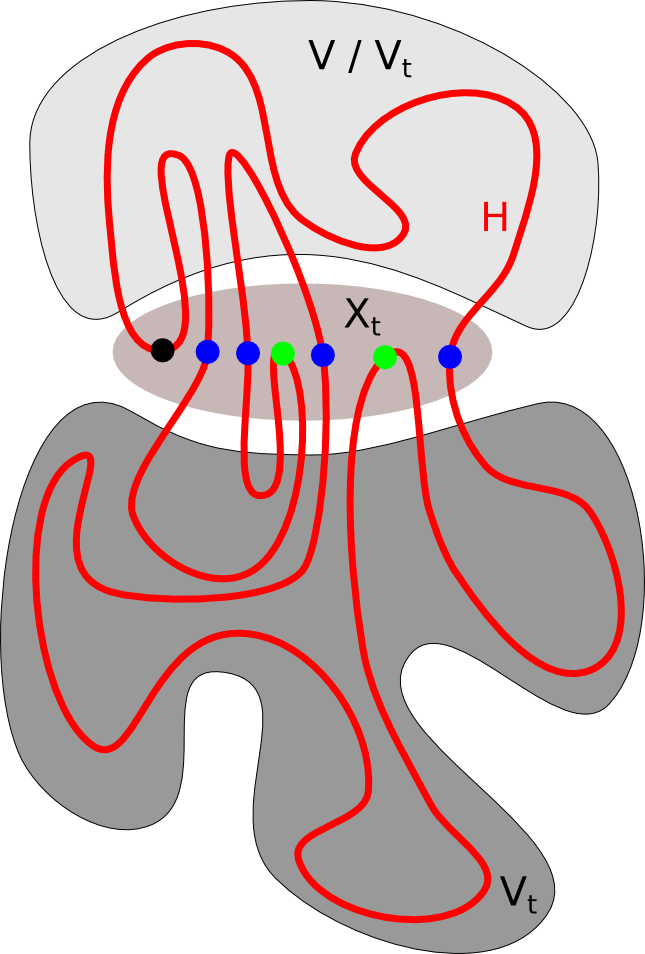
\includegraphics[scale=0.5]{src/figures/hcpd_hamilton_1.png}
        \caption{Représentation d'un cycle hamiltonien dans le graphe $G$ en fonction de $X_t$}
        \label{hcpd_h1}
    \end{center}
\end{figure}

\begin{figure}
    \begin{center}
        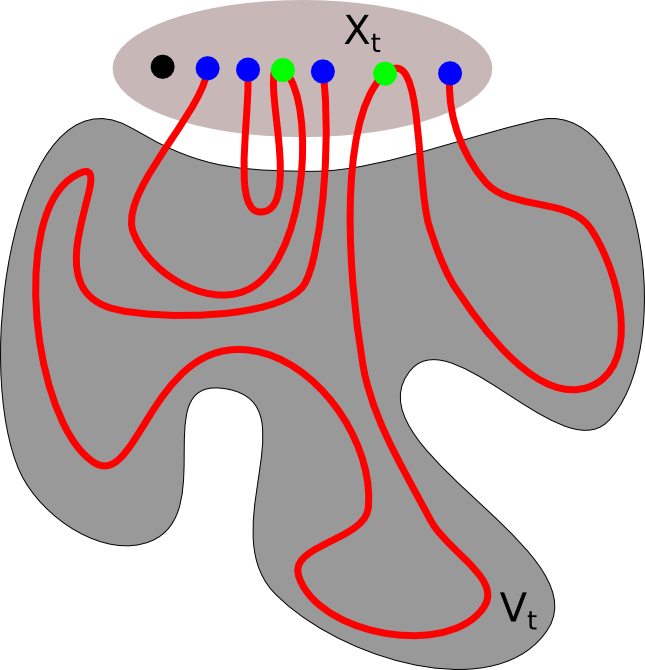
\includegraphics[scale=0.5]{src/figures/hcpd_hamilton_2.png}
        \caption{Représentation de la collection de chemins $H[V_t]$}
        \label{hcpd_h2}
    \end{center}
\end{figure}

\begin{figure}
    \begin{center}
        \hfill
        \subfloat[Collection $1$]{
            \label{fig:g1}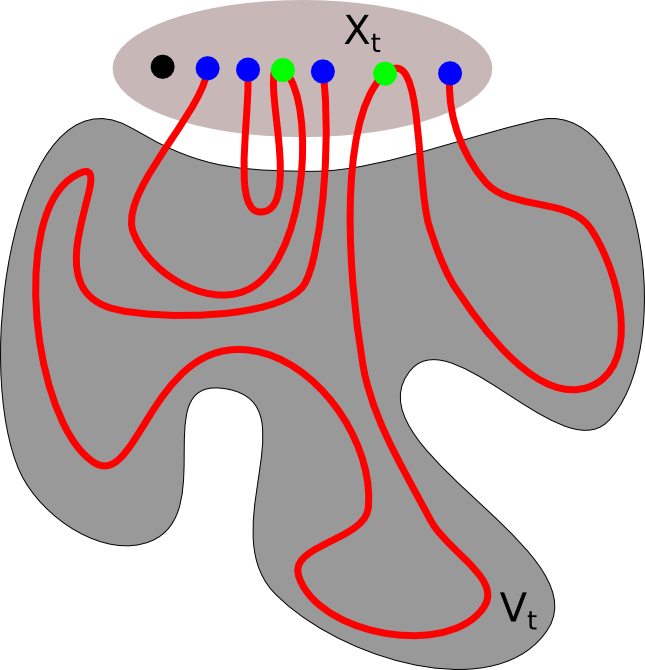
\includegraphics[scale=0.3]{src/figures/hcpd_hamilton_2.png}
        }
        \hfill
        \subfloat[Collection $2$]{
            \label{fig:g2}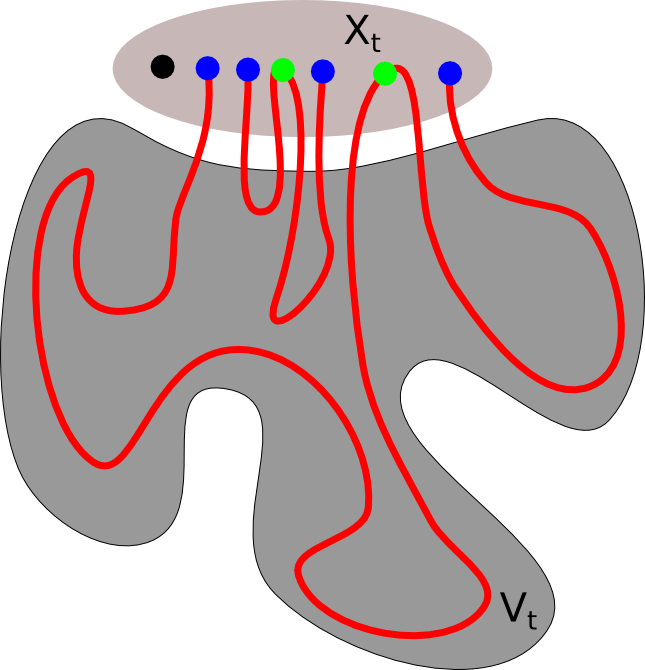
\includegraphics[scale=0.3]{src/figures/hcpd_hamilton_3g2.png}
        }
        \hfill
    \end{center}
    \caption{Deux collections de chemin différentes pour un même sac $X_t$}
    \label{hcpd_h3}
\end{figure}

\begin{figure}
    \begin{center}
        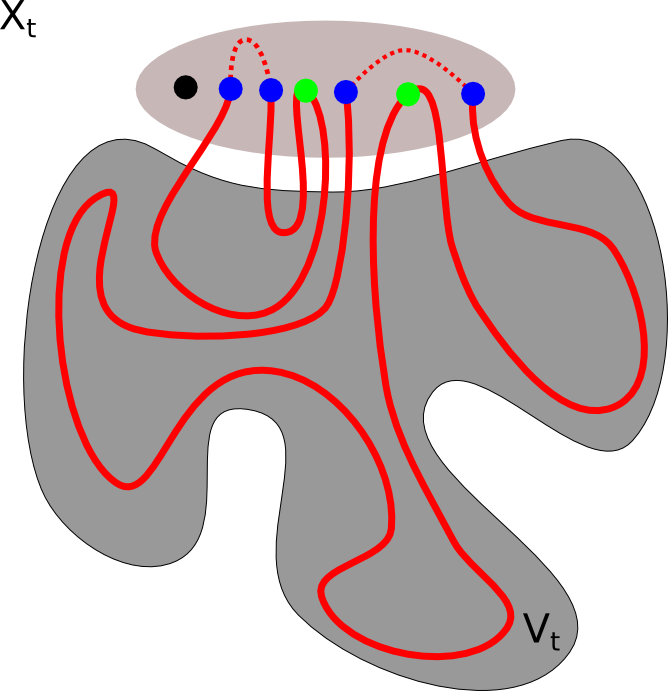
\includegraphics[scale=0.5]{src/figures/hcpd_hamilton_4.png}
        \caption{Représentation d'une solution partielle pour $X_t$}
        \label{hcpd_h1}
    \end{center}
\end{figure}

% }}}

%% }}}
%% {{{ ACTIONS SUR CHACUN DES NOEUDS
\section{La résolution du problème}

La question qui se pose à présent est de savoir comment calculer les solutions partielles d'un sac
$t \in T$. Il est possible de calculer ces solutions à partir des solutions des fils de $t$. C'est
ce que nous allons voir en étudiant les différents cas possibles.

\subsection{Le sac feuille}

Si $t$ est une feuille alors $X_t = \{x\}$ et $t$ n'a aucun fils. $x$ est donc obligatoirement de
degré $0$ et $(\{x\}, \emptyset, \emptyset, \emptyset)$ est une solution partielle.

\subsection{Le sac suppression}

$t$ est un sac suppression, il a donc un fils $t_f$ contenant $v$ tel que $X_{t_f} = X_t \cup
\{v\}$. 
\begin{nlemma}
    Soit $s_{t_f} = \pdsol{t_f}$ une solution partielle pour $t_f$ alors $s_t = (X_{t_f}^0, X_{t_f}^1,
    X_{t_f}^2\backslash\{v\}, M_{t_f})$ est une solution partielle pour $t$.
\end{nlemma}

\begin{proof}
    Remarquons de prime abord de $X_t$ est un séparateur de $G$ donc tout sommet $v$ n'appartenant
    pas à $X_t$ et appartenant à l'un des descendants $t'$ de $t$ est interne à $G_t$. Ainsi si $v$
    appartient à une solution partielle de $t_f$, alors $v \in X_{t_f}^2$. Le problème $\pdsol{t_f}$ pour
    $t_f$ est équivalent au problème $(X_t^0, X_t^1, X_t^2\backslash\{v\}, M_t)$ pour $t$, donc une
    solution partielle pour le problème pour $t$ existe si et seulement si le une solution partielle
    du problème pour $t_f$ existe.
\end{proof}

\subsection{Le sac ajout}

Si $t$ est un sac ajout, il a un fils $t_f$ et contient un sommet $v$ tel que $X_{t} = X_{t_f} \cup
\{v\}$.

Trois cas sont ici possibles, dépendant du degré du sommet $v$ rajouté.

\subsubsection{Le sommet $v$ appartient à $X_t^0$}

\begin{nlemma}
    $\pdsol{t_f}$ est une solution partielle pour $t_f$ si et seulement si $(X_{t_f}^0 \cup \{v\},
    X_{t_f}^1, X_{t_f}^2, M_{t_f})$ est une solution partielle pour $t$.
\end{nlemma}

La démonstration est évidente.

\subsubsection{Le sommet $v$ appartient à $X_t^1$}

\begin{nlemma}
    Il existe un sous problème $\pdsol{t_f}$ pour $t_f$ équivalent au sous problème $\pdsol{t}$ pour
    $t$.
\end{nlemma}

\begin{proof}
    Par définition du sac ajout, il existe un n\oe d $v$ appartenant à $X_t$ et pas à $X_{t_f}$,
    Puisque $X_{t_f}$ est un séparateur les voisins de $v$ appartiennent à $X_t$, or par hypothèse
    de départ, $v \in X_t^1$, donc $v$ a exactement un voisin $u$ dans $X_t$ et donc dans $X_{t_f}$.
    Décrivons deux cas :
    \begin{itemize}
        \item $u \in X_t^2$, dans ce cas $u \in X_{t_f}^1$ ce qui implique qu'il existe un sommet $w
            \in X_{t_f}^1$ tel que $(u,w) \in M_{t_f}$. On peut alors définir $M_t$ de la façon
            suivante : \[
                M_t = M_{t_f} \backslash \{(u,w)\} \cup \{(v,w)\}
            \]. C'est de cette façon que $u$ devient un n\oe ud interne dans $X_t$. Et donc le
            problème $\pdsol{t_f}$ est équivalent au sous problème $\pdsol{t}$ avec :
            \[
                \begin{array}{rcl}
                    X_t^0 & = & X_{t_f}^0 \\
                    X_t^1 & = & X_{t_f}^1 \backslash \{u\} \cup \{v\}\\
                    X_t^2 & = & X_{t_f}^2 \cup \{u\}\\
                \end{array}
            \]
        \item $u \in X_t^1$, dans ce cas, $u \in X_{t_f}^0$. Et donc le sous problème $\pdsol{t_f}$
            est équivalent au sous problème $\pdsol{t}$ avec :
            \[
                \begin{array}{rcl}
                    X_t^0 & = & X_{t_f}^0 \backslash \{u\} \\
                    X_t^1 & = & X_{t_f}^1 \cup \{u\}\\
                    X_t^2 & = & X_{t_f}^2\\
                    M_t = M_{t_f} \cup \{(u, v)\}\\
                \end{array}
            \]
    \end{itemize}
\end{proof}

\begin{ncorol}
    $\pdsol{f_t}$ est une solution partielle pour $t_f$, si et seulement si $(X_{t_f}^0, X_{t_f}^1
    \backslash \{u\} \cup \{v\},X_{t_f}^2 \cup \{u\},M_{t_f} \backslash \{(u,w)\} \cup \{(v,w)\})$
    et/ou $X_{t_f}^0 \backslash \{u\}, X_{t_f}^1 \cup \{u\}, X_{t_f}^2, M_{t_f} \cup \{(u, v)\})$ est
    une solution partielle pour $t$.
\end{ncorol}

\subsubsection{$v$ appartient à $X_t^2$}

\begin{nlemma}
    Il existe un sous problème $\pdsol{t_f}$ pour $t_f$ équivalent au sous problème $\pdsol{t}$ pour
    $t$.
\end{nlemma}

\begin{proof}
    Ce cas est très similaire au cas précédent à ceci près, $v$ est relié à deux sommets $u, w$ de
    $X_t$ pouvant chacun appartenir soit à $X_t^2$ (et dont à $X_{t_f}^1$) soit à $X_t^1$ (et donc à
    $X_{t_f}^0$).

    Détaillons donc les trois cas : \begin{enumerate}
        \item $u, w \in X_{t_f}^1$, dans ce cas $v$ relie $u$ et $w$ et il existe $k, l \in
            X_{t_f}^1$ tels que $(k, u), (l,w) \in M$. Il suffit donc d'enlever les
            couples $(k, u)$ et $(l,w)$ au couplage $M_{t_f}$ et de lui ajouter le couple $(k, l)$
            pour obtenir $M_t$.
        \item $u, w \in X_{t_f}^0$, dans ce cas encore, $v$ relie $u$ et $w$ faisant passer leur
            degré à $1$, on obtient donc $M_t$ en ajoutant le couple $(u,w)$ à $M_{t_f}$
        \item $u \in X_{f_t}^0$ et $w \in X_{f_t}^1$, dans ce cas, il existe $k \in X_{f_t}^1$ tel
            que le couple $(k,w) \in M_{t_f}$. Il suffit alors de supprimer $(k,w)$ à $M_{t_f}$ et
            de lui ajouter le couple $(k, u)$ pour obtenir $M$.
    \end{enumerate}
\end{proof}

\begin{ncorol}
    $\pdsol{f_t}$ est une solution partielle pour $t_f$ si et seulement si au moins l'une des trois
    propositions suivantes est une solution partielle pour $t$ :
    \begin{enumerate}
        \item $(X_{t_f}^0, X_{t_f}^1 \backslash \{u, w\}, X_{t_f}^2 \cup \{u, v, w\}, M \backslash
            \{(k, u), (l, w)\} \cup \{(k, l)\})$
        \item $(X_{t_f}^0 \backslash \{u, w\}, X_{t_f}^1 \cup \{u, w\}, X_{t_f}^2 \cup \{v\}, M \cup
            \{(u, w)\})$
        \item $(X_{t_f}^0 \backslash \{u\}, X_{t_f}^1 \backslash \{w\} \cup \{u\}, X_{t_f}^2 \cup
            \{v, w\}, M \backslash \{(k, w)\} \cup \{(k, u)\})$
    \end{enumerate}
\end{ncorol}
        
\subsubsection{Le sac fusion}

$t$ est un sac fusion il possède donc deux fils $t_1$ et $t_2$ tels que $X_t = X_{t_1} = X_{t_2}$.
L'opération à réaliser est alors un fusion des solutions de $t_1$ et $t_2$ tout en vérifiant la
validité des solutions obtenues.

\begin{nlemma}
    Le sous problème $\pdsol{t}$ associé à $t$ admet au moins une solution si et seulement si il
    existe deux sous problème $\pdsol{t_1}$ et $\pdsol{t_2}$ associés à $t_1$ et $t_2$ vérifiant les
    conditions suivantes :
    \begin{enumerate}
        \item $X_{t_1}^2 \subseteq X_{t_2}^0$ et $X_{t_1}^1 \suseteq X_{t_2}^1 \cup X_{t_2}^0$
        \item $X_{t_2}^2 \subseteq X_{t_1}^0$ et $X_{t_2}^1 \suseteq X_{t_1}^1 \cup X_{t_1}^0$
        \item $M_{t_1} \cup M_{t_2}$ ne contient pas de cycle
    \end{eumerate}
\end{nlemma}

%% }}}
% {{{ VALIDITE
% }}}
%% {{{ COMPLEXITE
%% }}}
% }}}
